\begin{figure*}[t]
    \centering
    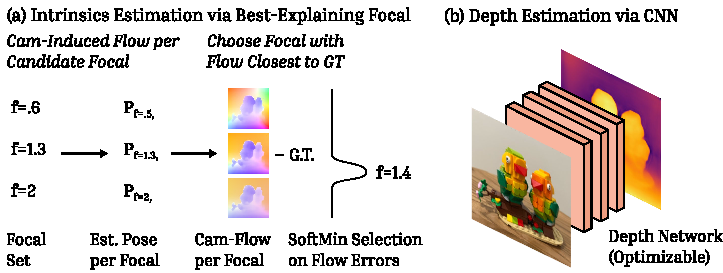
\includegraphics[width=\linewidth,]{figures/pdfs/focal_and_depth_est_fix_compressed.pdf}
    \caption{In (a) we illustrate our implicit focal length formulation, which considers a set of candidate focal lengths, assigns each one an error score, and softly selects the focal length with the lowest error. To calculate the error score for a focal length, we use that focal length to estimate a pose, and then compare the resulting pose-induced optical flow to the ground truth optical flow. In (b) we illustrate that we parameterize depth via the output of a monocular depth prediction CNN. }
    \label{fig:focal_and_depth}
\end{figure*}

\section{Experiment Details}

\subsection{Image Resolution}

To manage computational cost (our current implementation loads the entire video into memory), we compute optical flow and point tracks at a resolution of around 700,000 pixels, then perform FlowMap optimization at 1/16th the resolution.

\subsection{Hyperparameters}

We train for 2000 steps using Adam and use a learning rate of 3e-5.
For the pose-as-variable experiments, we choose Euler angles as the parameterization of the rotation matrix.

\subsection{Pre-Training Details}

Before performing per-scene fine-tuning, we found it useful to learn a large-scale prior for better initialization.
We use the same FlowMap loss formulation but train it on datasets of videos (instead of optimizing on a single scene).
We use videos from CO3D, Real Estate 10K, and KITTI for pretraining.
Note that we only use the raw videos from these datasets (no intrinsics, poses, or sparse geometry).
